\documentclass[compress]{beamer}
\usepackage{ifthen,verbatim}

\newcommand{\isnote}{}

%% Uncomment this to get annotations
\def\notes{\addtocounter{page}{-1}
           \renewcommand{\isnote}{*}
           \beamertemplateshadingbackground{lightgray}{lightgray}
           \begin{frame}
           \frametitle{Notes for the previous page (page \insertpagenumber)}
           \itemize}
\def\endnotes{\enditemize
	      \end{frame}
              \beamertemplateshadingbackground{white}{white}
              \renewcommand{\isnote}{}}

%% Uncomment this to not get annotations
%% \def\notes{\comment}
%% \def\endnotes{\endcomment}

\setbeamertemplate{navigation symbols}{}
\setbeamertemplate{headline}{\includegraphics[height=1 cm]{../cmslogo} \hspace{0.1 cm} \includegraphics[height=1 cm]{../tamulogo} \hfill
\begin{minipage}{9 cm}
\vspace{-0.75 cm} \small
\begin{center}
\ifthenelse{\equal{\insertpagenumber}{1}}{}{\insertsection}
\end{center}
\end{minipage} \hfill
\begin{minipage}{1 cm}
\vspace{-0.75 cm} \small
\begin{flushright}
\ifthenelse{\equal{\insertpagenumber}{1}}{}{\insertpagenumber\isnote/\pageref{numpages}} \mbox{ }
\end{flushright}
\end{minipage}}

\begin{document}
\begin{frame}
\begin{center}
\textcolor{blue}{\Large Track-based Alignment of the Muon System}

\vfill
Jim Pivarski, Alexei Safonov, Dmitry Yakorev

{\small Texas A\&M University}

\vfill
Karoly Banicz

{\small Purdue University}

\vfill
16 June, 2007
\end{center}
\end{frame}

% Infrastructure for real-time alignments
% 
%    Data path and triggers: Alexei's slide
% 
%    Muon AlCaReco format
% 
%    Monitoring
% 
%        Low-level monitoring
% 
%        Javier's analyzer
% 
% Survey measurements -> constraints
% 
%    DT constraints (talk to Pablo)
% 
%    CSC constraints
% 
% Testing the system: MTCC and MC
% 
% MTCC
% 
%    Karoly's (re-)discovery of layer offsets in MTCC
% 
%    Reproduce in AlignmentProducer/HIP
% 
%    Preliminary results, need more data, more robustness
% 
% MC: debugging the procedure
% 
%    List of ways this is more realistic/ambitious
% 
%    Two major approaches: lowbias and standalone
% 
%    lowbias: between tracker-to-muon and globalMuon (show residuals)
% 
%    standalone: it converges!
% 
%    same for lowbias: converges much faster
% 
% MC results
% 
%    alignment corrections/output
% 
%    three figures of merit: core sigma, RMS, |max|
% 
%    as a function of iteration (colorful!)
% 
%    as a function of integrated luminosity
% 
%    layer alignments: same treatment
% 
% Systematics studies
% 
%    list of candidates
% 
%    lowbias's dependence on tracker alignment
% 
%    dependence on fitting constraints: preview of survey constraint
%  
% Summary
   
\section*{Track-based Alignment --- Jim Pivarski}

\begin{frame}
\frametitle{Introduction and Overview}
\begin{itemize}\setlength{\itemsep}{0.5 cm}
\item Development of infrastructure: ready for CSA07
\item Survey measurements (used as constraints for track-based alignment)
\item MC: developing the procedure
\item Alignment results in MC
\item MTCC: early attempts on real data
\end{itemize}
\end{frame}

\begin{notes}
\item You have downloaded the {\it annotated} version of this talk.  I
didn't show these notes (grey pages) visually when I presented the
talk, though I should have made the following points orally.

\vspace{0.2 cm}
If you are following the presentation as I am making it, please
download the other version (should say ``download-this-one'') which is the
same, minus the grey pages.

\vfill
\item This will be a general overview, but with a focus on A\&M work
\item The majority of this talk will be about developing and testing the procedure with MC
\end{notes}

\begin{frame}
\frametitle{Infrastructure}
\begin{columns}
\column{0.7\linewidth}
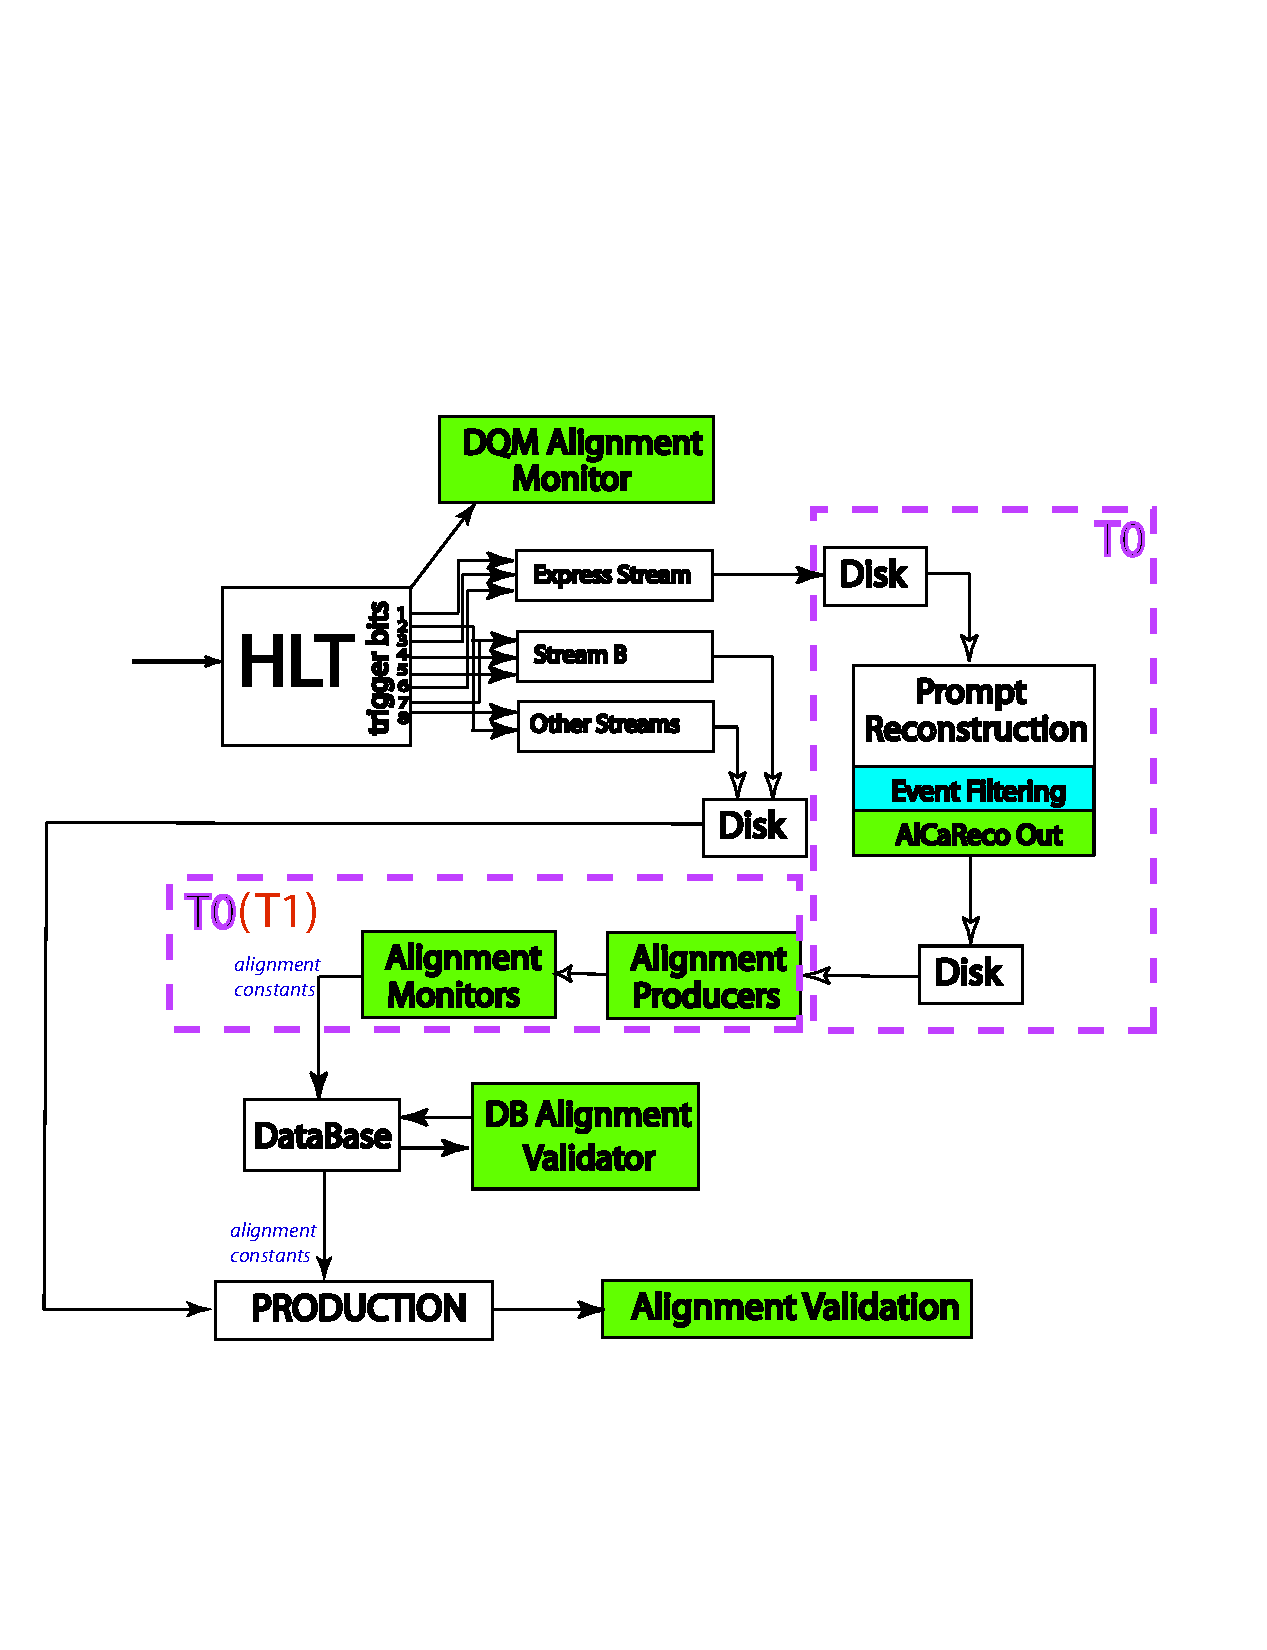
\includegraphics[width=1.2\linewidth]{realplots/alexeis_graph2.png}
\column{0.3\linewidth}
\begin{itemize}
\item Defined data path and triggers 
\item Defined data format for muon alignment stream
\item Developed monitoring tools
\item Ready for CSA07
\end{itemize}
\end{columns}
\end{frame}

\begin{notes}
\item We plan to get muons from all available triggers (single-, di-muon\ldots)
\item Express stream is 25\% of all data (in early running), very inclusive
\item We have completed the pipeline from express stream, through
prompt reconstruction, AlCaReco, Alignment Producers, Alignment
Monitors, to database (SQLite file, at least).
\item DQM Monitor, DB Validator and the last stage of Alignment
Validation (external legs on this graph) still need work
\end{notes}

\begin{frame}
\frametitle{Alignment Monitor Tool}
\begin{enumerate}
\item CommonAlignmentMonitor: general plotting package integrated into AlignmentProducer
\begin{itemize}
\item Manages iteration, collection after parallel processing
\end{itemize}
\item AlignmentMonitorMuonHIP outputs histograms for every chamber (or every layer): residuals versus everything
\item pyROOT script merges histograms on the fly
\end{enumerate}
\begin{center}
\includegraphics[width=0.8\linewidth]{realplots/monitoring_tool}
\end{center}
\begin{itemize}
\item Offline Alignment Validation, the last step in monitoring, sees changes in $p_T$, $Z'$ resolution (Javier Fernandez)
\end{itemize}
\end{frame}

\begin{notes}
\small
\item Command for the featured plot: ``r.select(lambda c, h: not c.barrel and h.GetEntries() $>$ 0)''
\item Can pass arbitrary Python functions to select by chamber information (c) or histogram features (h)
\item Almost as much versatility as an ntuple, this tool will allow us to
``zoom in'' on alignment problems, to understand specific outliers and
allow human decision-making in early data
\item ROOT file sizes are $\sim$10 MB per iteration
\item A link to information about Javier's analyzer: http://indico.cern.ch/conferenceDisplay.py?confId=13742
\item Due to the way we do track refitting, the integrated monitor is
sensitive to updated residuals but not updated track parameters.
Thus, we can use AlignmentMonitorMuonHIP to see narrowing
residuals/$\chi^2$, and then re-reconstruct from scratch with Javier's
analyzer to see the change in $p_T$ distributions, the $Z'$ peak,
Drell-Yan seepage, etc.
\end{notes}

\begin{frame}
\frametitle{Survey measurements}
\begin{itemize}
\item This is the initial geometry used in track-based alignment
\item Can also be used as a constraint on track-based alignment
\item Positions of optical targets are measured by photogrammetry and later transformed into chamber positions/orientations
\item CSC measurement is good; transformation contains an error
\end{itemize}

\vfill
\mbox{\hspace{-1.5 cm} \begin{tabular}{p{0.6\linewidth} p{0.5\linewidth}}
\begin{minipage}{\linewidth}
  \begin{center}
    \includegraphics[width=3 cm]{realplots/dmitry1}
  \end{center}
\end{minipage} &
\begin{minipage}{\linewidth}
  \begin{center}
    \includegraphics[width=3 cm]{realplots/dmitry2}
  \end{center}
\end{minipage} \\
\begin{minipage}{\linewidth}
  \begin{center}
    Measurement resolution: $\sim$300 $\mu$m
  \end{center}
\end{minipage} &
\begin{minipage}{\linewidth}
  \begin{center}
    Consistency check: $\sim$1 mm
  \end{center}
\end{minipage}
\end{tabular}}
\end{frame}

\begin{notes}
\item Survey constraint implemented for tracker alignment, not yet tested for muon alignment, but we use the same infrastructure
\item Pablo Martinez Ruiz del Arbol has transformed DT survey measurements into chamber orientations, but has not yet uploaded to the database
\item Dmitry Yakorev has transformed CSC survey measurements into
chamber orientations and performed the consistency check that revealed
the error.  He's dividing-and-conquering the problem now\ldots
\end{notes}

\begin{frame}
\begin{center}
\huge \textcolor{blue}{Testing the alignment system in MC}
\end{center}
\end{frame}

\section*{Track-based alignment in MC --- Jim Pivarski}

\begin{frame}
\frametitle{MC: developing the procedure}
\begin{itemize}\setlength{\itemsep}{0.25 cm}
\item More realistic than this spring's test-run (presented at UCLA)

\begin{itemize}\setlength{\itemsep}{0.25 cm}
\item Large datasets: 10 pb$^{-1}$ and 100 pb$^{-1}$ of muons from $W$ and $Z$ (simulated by $Z$ only)
\item More ambitious precision goals (200 $\mu$m, rather than 1 cm)
\item Random misalignments with SurveyOnlyScenario (rather than moving all chambers in the same direction)
\item First attempt at muon system self-measurement
\end{itemize}

\item Two major approaches, developed simultaneously

\begin{itemize}\setlength{\itemsep}{0.25 cm}
\item Align the muon system to the tracker (globalMuons)
\begin{itemize}
\item converges more quickly
\end{itemize}

\item Align the muon system to itself (standAloneMuons)
\begin{itemize}
\item independent of the tracker
\end{itemize}
\end{itemize}
\end{itemize}
\end{frame}

\begin{frame}
\frametitle{Aligning to the tracker}
\begin{itemize}
\item Residuals from globalMuons have two peaks per chamber, due to track-fitting bias
\end{itemize}

\begin{tabular}{p{0.4\linewidth} p{0.6\linewidth}}
\begin{minipage}{\linewidth}
\includegraphics[width=3 cm, angle=90]{realplots/bias_residual_globalMuon}
\end{minipage} &
\begin{minipage}{\linewidth}
\begin{center}
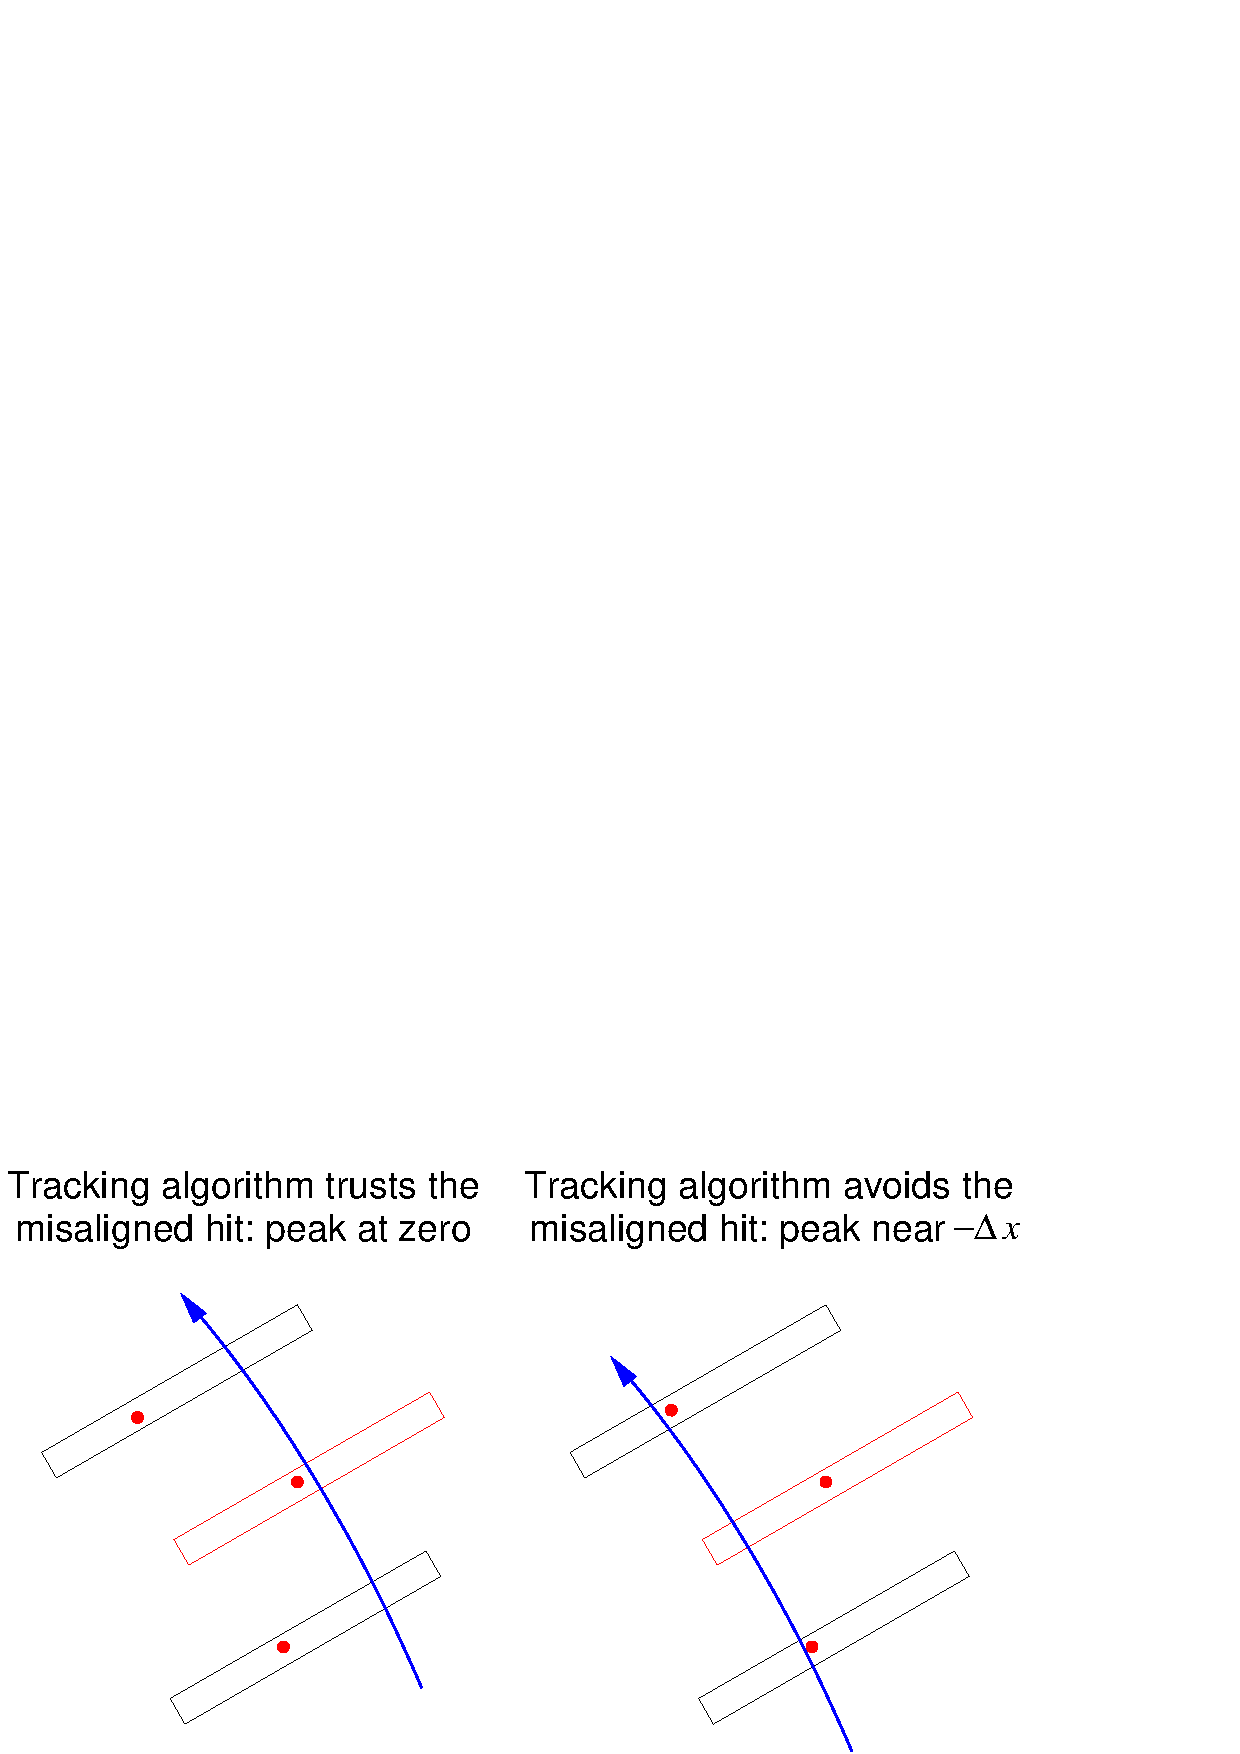
\includegraphics[height=3 cm]{realplots/two_cases.pdf}
\end{center}
\end{minipage} \\
 & \\
\begin{minipage}{\linewidth}
\includegraphics[width=3 cm, angle=90]{realplots/bias_residual_tracker-to-muon}
\end{minipage} &
\begin{minipage}{\linewidth}
\begin{itemize}
\item Simply extrapolating a tracker track into the muon system removes the bias, but at a severe resolution cost (note wider scale)
\item Neither is optimal
\end{itemize}
\end{minipage}
\end{tabular}
\end{frame}

\begin{notes}
\item The tracker-to-muon extrapolation is what I presented in my last EMU talk at UCLA
\item Alignment resolution was $\sim$4 mm
\end{notes}

\begin{frame}
\frametitle{The ``lowbias'' method}
\begin{itemize}
\item Re-fit globalMuon tracks with inflated hit uncertainties in the muon system
\item Resulting tracks are determined mostly by the silicon tracker, but they ``know'' about scattering in the muon system
\end{itemize}
\begin{center}
\includegraphics[height=0.7\linewidth, angle=90]{realplots/bias_residual_lowbias}
\end{center}
\end{frame}

\begin{notes}
\item The tall peak at 1 cm is the misalignment, small peak at 0 is due to bias
\item Usually converges in one iteration
\end{notes}

\begin{frame}
\frametitle{The ``standalone'' method}
\begin{itemize}
\item standAloneMuons have the two-peak structure in residuals, and therefore need to iterate to decouple track-fitting from chamber alignment
\item With a $|\mbox{residuals}| <$ 5 cm cut, this method shows clear convergence for most chambers:
\begin{center}
\includegraphics[height=0.48\linewidth, angle=90]{realplots/standalone_converges}
\includegraphics[height=0.48\linewidth, angle=90]{realplots/standalone_residuals}
\end{center}

\item We are keenly interested in saving the tails\ldots
\end{itemize}
\end{frame}

\begin{notes}
\item We need to study the outliers!  Figure out what's happening to
the tails!  Find a way to diagnose it in data, also (shape of residual
distribution?)

\item Muon alignment is especially important for keeping Drell-Yan
backgrounds from smearing into high dimuon-mass channels for New
Physics.  We therefore care very much about the higher moments of the
$p_T$ distribution, which is to say, alignment outliers.
\end{notes}

\begin{frame}
\frametitle{The same plots for ``lowbias''}
\begin{center}
\includegraphics[height=0.48\linewidth, angle=90]{realplots/lowbias_converges}
\includegraphics[height=0.48\linewidth, angle=90]{realplots/lowbias_residuals}
\end{center}
\begin{itemize}
\item Converges in one iteration
\item Beyond that most chambers are stable, but a few DTs wander
\item There's also a cumulative problem with hit efficiency
\end{itemize}
\end{frame}

\section*{Track-based alignment results --- Jim Pivarski}

\begin{frame}
\frametitle{Alignment Results (10 pb$^{-1}$)}
\begin{itemize}\setlength{\itemsep}{0.25 cm}
\item Starting from MuonSurveyOnlyScenario: positions misaligned 2.5 mm, $\phi_z$ misaligned 0.25 mrad

\item Five degrees of freedom in alignment: $x$, $y$, $\phi_x$, $\phi_y$, $\phi_z$

\item Accuracy: \textcolor{blue}{one iteration lowbias}, \textcolor{red}{ten iterations standalone}
\begin{center}
\begin{tabular}{c c}
\includegraphics[height=0.4\linewidth, angle=90]{realplots/x_positions} &
\includegraphics[height=0.4\linewidth, angle=90]{realplots/y_positions} \\
$x_{\mbox{\scriptsize aligned}} - x_{\mbox{\scriptsize true}}$ (cm) &
$y_{\mbox{\scriptsize aligned}} - y_{\mbox{\scriptsize true}}$ (cm)
\end{tabular}
\end{center}

\item Precision: alignment uncertainties are still underestimated by a factor of 3--4
\end{itemize}
\end{frame}

\begin{frame}
\frametitle{Figures of merit}
\vspace{-0.75 cm}
\begin{columns}
\column{0.4\linewidth}
\begin{enumerate}
\item $\sigma$ of core Gaussian (best-measured chambers)
\item RMS, cut at 1 cm
\item $|\mbox{max}|$ (worst outlier)
\end{enumerate}

\column{0.6\linewidth}
\begin{center}
\begin{tabular}{c | c c c}
790 chambers & core $\sigma$ & RMS & $|\mbox{max}|$ \\\hline
\textcolor{blue}{lowbias $x$} & \textcolor{blue}{50} & \textcolor{blue}{280} & \textcolor{blue}{4500} \\
\textcolor{blue}{lowbias $y$} & \textcolor{blue}{270} & \textcolor{blue}{860} & \textcolor{blue}{6000} \\
\textcolor{red}{standalone $x$} & \textcolor{red}{50} & \textcolor{red}{1040} & \textcolor{red}{$\infty$} \\
\textcolor{red}{standalone $y$} & \textcolor{red}{290} & \textcolor{red}{1540} & \textcolor{red}{34000} \\
\end{tabular}
\mbox{ } \hfill microns
\end{center}

\end{columns}

\vfill
\includegraphics[height=0.48\linewidth, angle=90]{realplots/lowbias_fit}
\includegraphics[height=0.48\linewidth, angle=90]{realplots/standalone_fit} \\
\end{frame}

\begin{notes}
\small
\item Fits are purely Gaussian on a restricted range: $\pm$100 $\mu$m for $x$ and $\pm$500 $\mu$m for $y$.
\item The RMS that I quote is cut at 1 cm (as stated on the previous page).  The RMS that ROOT reports in its statistics boxes is cut to the current window width, and I zoom into some of the plots for detail.  Therefore, ROOT sometimes a different RMS in its statistics box than I quote in the table and in plots on the next few pages.  I was careful to always use a 1 cm cut in all the numbers I report!
\item $|\mbox{max}|$ is extremely twitchy, as you may imagine.  These $|\mbox{max}|$ numbers are dominated by the few chambers that diverge, so the numerical value doesn't have a precise meaning, it's only a guide to say that I still have divergent chambers.  It will become more useful when I fix that DT problem.
\item For the sake of the table, I selected the largest ``reasonable'' value.  A few values were 5098450298475e+4598; I skipped those.  In the case labelled with an $\infty$, there wasn't a clear break between reasonable and unreasonable.
\end{notes}

\begin{frame}
\frametitle{Figures of merit versus iteration}
\begin{columns}
\column{0.48\linewidth}
\begin{center}
\includegraphics[width=\linewidth]{realplots/x_width_vsiter_lowbias}
\end{center}
\column{0.48\linewidth}
\begin{center}
\includegraphics[width=\linewidth]{realplots/x_width_vsiter_standalone}
\end{center}
\end{columns}
\begin{itemize}
\item Core $\sigma$ largely unchanged after first iteration
\item standalone method requires 7 iterations
\end{itemize}
\end{frame}

\begin{frame}
\frametitle{Figures of merit versus integrated luminosity}
\begin{columns}
\column{0.48\linewidth}
\begin{center}
\includegraphics[width=\linewidth]{realplots/lowbias_width_vsevents}
\end{center}
\column{0.48\linewidth}
\begin{center}
\includegraphics[width=\linewidth]{realplots/standalone_width_vsevents}
\end{center}
\end{columns}
\begin{itemize}
\item lowbias reaches sensitivity limit between 10 and 100 pb$^{-1}$
\item standalone technique reaches limit below 10 pb$^{-1}$
\end{itemize}
\end{frame}

\begin{notes}
\item That second plot looks very strange because the high-luminosity
point actually has less resolution than the low luminosity point.  If
you look at the corresponding resolution vs.\ iteration, you'll see
that this difference is in the noise.  If I assigned errorbars, the
points would be consistent.

\includegraphics[width=0.5\linewidth]{realplots/x_width_vsiter_standalone_100}
\end{notes}

%% \begin{frame}
%% \frametitle{motivation for layer-by-layer}

%% \end{frame}

%% \begin{frame}
%% \frametitle{Results for layer-by-layer alignments}

%% \only<1>{\includegraphics[width=0.48\linewidth]{cartoons/layer_x_positions}}
%% \only<2>{\includegraphics[width=0.48\linewidth]{cartoons/layer_y_positions}}
%% \only<1>{\includegraphics[width=0.48\linewidth]{cartoons/layer_x_residuals}}
%% \only<2>{\includegraphics[width=0.48\linewidth]{cartoons/layer_y_residuals}}

%% left: \only<1>{$x_{\mbox{\scriptsize aligned}} - x_{\mbox{\scriptsize true}}$}\only<2>{$y_{\mbox{\scriptsize aligned}} - y_{\mbox{\scriptsize true}}$} \hfill right: \only<1>{$x$}\only<2>{$y$} residuals

%% \vfill
%% \begin{itemize}
%% \item Mystery: standalone appears to be much better than lowbias.  Perhaps lowbias needs multiple iterations for layer-by-layer alignments?
%% \end{itemize}
%% \end{frame}

%% \begin{frame}
%% \frametitle{Layer figures of merit versus iteration}
%% \begin{columns}
%% \column{0.48\linewidth}
%% \begin{center}
%% \includegraphics[width=\linewidth]{cartoons/merit_vs_iteration}

%% lowbias
%% \end{center}
%% \column{0.48\linewidth}
%% \begin{center}
%% \includegraphics[width=\linewidth]{cartoons/merit_vs_iteration}

%% standalone
%% \end{center}
%% \end{columns}
%% \end{frame}

%% \begin{frame}
%% \frametitle{Layer figures of merit versus integrated luminosity}
%% \begin{columns}
%% \column{0.48\linewidth}
%% \begin{center}
%% \includegraphics[width=\linewidth]{cartoons/merit_vs_events}

%% lowbias
%% \end{center}
%% \column{0.48\linewidth}
%% \begin{center}
%% \includegraphics[width=\linewidth]{cartoons/merit_vs_events}

%% standalone
%% \end{center}
%% \end{columns}
%% \end{frame}

\begin{frame}
\frametitle{Planned systematics studies}
\begin{itemize}\setlength{\itemsep}{0.25 cm}
\item \textcolor{blue}{Dependence of lowbias on tracker alignment \hfill in progress}
\item \textcolor{blue}{Dependence on fitting constraints \hfill in progress}
%% \item \textcolor{blue}{Dependence of lowbias on tracker alignment}
%% \item \textcolor{blue}{Dependence on fitting constraints}
\item Dependence on survey constraints
\begin{itemize}
\item obtain survey geometries and apply constraints
\end{itemize}
\item Dependence on tracking algorithm
\begin{itemize}
\item Uncertainty in distribution of material
\item Uncertainty in $\vec{B}(\vec{x})$
\end{itemize}
\item Background studies in CSA07
\begin{itemize}
\item Multiple scattering in low-$p_T$ muons
\begin{itemize}
\item Alignment with $J/\psi\to\mu\mu$
\end{itemize}
\item Effect of fake muons in the alignment stream
\begin{itemize}
\item Obtain realistic background samples from CSA07
\item Finalize track quality cuts
\end{itemize}
\end{itemize}
\end{itemize}
\end{frame}

\begin{notes}
%% \item On the previous page, \textcolor{blue}{blue} means that I have
%% already taken a look at this systematic, and I'll show it in the
%% upcoming pages

\item We already have a small $J/\psi$ sample that we can work with.
Due to inefficiencies of low-$p_T$ muons, it probably won't be
possible to do an alignment with these $J/\psi$s, but we can at least
compare the widths of the residual distributions, and scale from that.
\end{notes}

\section*{Track-based alignment in MTCC --- Jim Pivarski}

\begin{frame}
\begin{center}
\huge \textcolor{blue}{Testing the alignment system in MTCC}
\end{center}
\end{frame}

\begin{frame}
\frametitle{Karoly Banicz's (re-)discovery of layer offsets}
\begin{columns}
\column{0.3\linewidth}
\begin{itemize}
\item Agrees with FAST site measurements
\item \textcolor{blue}{We want to reproduce this study in AlignmentProducer}
\end{itemize}
\column{0.7\linewidth}
\includegraphics[width=\linewidth]{realplots/karolys_layers}
\end{columns}

\begin{center}
\begin{tabular}{c | c c c}
120 aligned layer positions & mean & stdev & $|\mbox{max}|$ \\ \hline
$x$ & -55 $\mu$m & 190 $\mu$m & 670 $\mu$m \\
$y$ & 110 $\mu$m & 330 $\mu$m & 1.2 mm \\
$\phi_z$ & 0.01 mrad & 0.04 mrad & 0.15 mrad
\end{tabular}
\end{center}
\end{frame}

\begin{frame}
\frametitle{Preliminary MTCC alignment with AlignmentProducer}
\begin{itemize}\setlength{\itemsep}{0.25 cm}
\item Alignment attempts were beset by random crashes
\item A single standalone iteration survived; not enough for a reliable alignment, but enough for order-of-magnitude

\vspace{0.25 cm}
\begin{center}
\begin{tabular}{c | c c c}
102 semi-aligned layer positions & mean & stdev & $|\mbox{max}|$ \\ \hline
$x$ & 8 $\mu$m & \textcolor{blue}{192 $\mu$m} & 440 $\mu$m
\end{tabular}
\end{center}

\vspace{0.25 cm}
\item in rough agreement with Karoly's results

\vfill
\item We'll need more data and more robust computation
\item Likely to get both with MTCC 1\_5\_0 re-reconstruction
\end{itemize}
\end{frame}

\begin{frame}
\frametitle{How well can we do layer-by-layer alignments anyway?}

\begin{center}
\mbox{Back to MC\ldots} \mbox{\begin{minipage}{0.6\linewidth}
\begin{tabular}{c | c c c}
3920 layers & core $\sigma$ & RMS & $|\mbox{max}|$ \\\hline
\textcolor{blue}{lowbias $x$} & \textcolor{blue}{50} & \textcolor{blue}{1630} & \textcolor{blue}{6600} \\
\textcolor{blue}{lowbias $y$} & \textcolor{blue}{360} & \textcolor{blue}{1830} & \textcolor{blue}{13000} \\
\textcolor{red}{standalone $x$} & \textcolor{red}{60} & \textcolor{red}{1720} & \textcolor{red}{6600} \\
\textcolor{red}{standalone $y$} & \textcolor{red}{380} & \textcolor{red}{1970} & \textcolor{red}{6400} \\
\end{tabular}
\mbox{ } \hfill microns
\end{minipage}}
\end{center}
\vfill
\includegraphics[height=0.48\linewidth, angle=90]{realplots/layer_x_lowbias_fit}
\includegraphics[height=0.48\linewidth, angle=90]{realplots/layer_x_standalone_fit} \\
\end{frame}

\begin{frame}
\begin{center}
\includegraphics[height=0.48\linewidth, angle=90]{realplots/layer_x_width_vsiter_standalone.pdf}

\includegraphics[height=0.48\linewidth, angle=90]{realplots/layer_lowbias_width_vsevents.pdf}
\includegraphics[height=0.48\linewidth, angle=90]{realplots/layer_standalone_width_vsevents.pdf}
\end{center}
\end{frame}

\section*{Track-based Alignment --- Jim Pivarski}

\begin{frame}
\frametitle{Summary}
\begin{itemize}\setlength{\itemsep}{0.25 cm}
\item Overall scheme and infrastructure components are now mature
\item Entering the era of precision alignment studies
\item Procedure is ready for CSA07, some updates need to be checked into CVS
\item We have taken a first glance at MTCC data and are ready to apply our software to 1\_5\_0 re-reconstructed data
\item Concrete list of systematics studies planned for CSA07
\item The software is available for cosmic ray/beam halo studies\ldots
\item We're starting to write a CMS Note
\end{itemize}
\label{numpages}
\end{frame}

\section*{Backup slides --- Jim Pivarski}

\begin{frame}
\begin{center}
\huge \textcolor{blue}{Backup Slides}
\end{center}
\end{frame}

\begin{frame}
\frametitle{Dependence of lowbias on tracker alignment}
\begin{itemize}\setlength{\itemsep}{0.5 cm}
\item The lowbias technique aligns the muon system using tracks which were fitted to the silicon tracker
\item How does muon alignment depend on the tracker's alignment?

\vfill
\begin{center}
\includegraphics[height=0.48\linewidth, angle=90]{realplots/lowbias_trackergeom_x}
\includegraphics[height=0.48\linewidth, angle=90]{realplots/lowbias_trackergeom_y}
\end{center}

\item Differences between alignment scenarios appears to be weak
\end{itemize}
\end{frame}

\begin{frame}
\frametitle{Dependence on fitting constraints}
\begin{itemize}\setlength{\itemsep}{0.5 cm}
\item Reducing the number of degrees of freedom should improve convergence

\begin{center}
\includegraphics[height=0.48\linewidth, angle=90]{realplots/lowbias_constraints_x}
\includegraphics[height=0.48\linewidth, angle=90]{realplots/lowbias_constraints_y}
\end{center}

\item Again, dependence is weak
\end{itemize}
\end{frame}

\begin{notes}
\item Both of the last two studies, the dependence on tracker
alignment and on fitting constraints, seem pretty conclusive, but I'm
not sure how to interpret the statistics.
\item At face value, it looks
like there are no statistically significant differences between
anything, though the histograms are not exactly the same (which would
be evidence of a mistake).
\item But they all began with the same misalignment (at least they
were supposed to!) and aligned on the same data, so they're not
statistically independent.
\item There are several follow-up studies I can do: (a) make sure that
the initial misalignments are the same, (b) follow each chamber
individually in the various cases.
\end{notes}

\begin{frame}
\frametitle{Are the MTCC layer offsets real?}
\begin{itemize}
\item Or are we under-reporting our uncertainties?
\item Can we find a pair of divergent layers in the same chamber?
\begin{center}
\includegraphics[height=0.7\linewidth, angle=90]{realplots/extremum}
\end{center}
\item \textcolor{red}{red} is layer 3, \textcolor{blue}{blue} is layer 6 in chamber 27 in ME+3/2
\end{itemize}
\end{frame}

\begin{notes}
\item This is not completely convincing because I haven't controlled
for the possibility that the whole chamber hasn't rotated, in, say,
$\phi_y$.  This can lead to the $x$ projection showing a discrepancy
between layers.  There could be rock-solid evidence of $\sim$200
$\mu$m misalignment here (other than, of course, Karoly's alignment
calculation and its agreement with FAST measurements), but it will
take more work to rule out other hypotheses.
\end{notes}

\end{document}
